\chapter{Horizontal-gene transfer as a source of novel sRNAs in \textit{Salmonella} Typhimurium}
\label{chap:sal_sRNA}
\section{Preface}

Despite their important role in gene regulation, studies of the evolutionary dynamics and origins of bacterial sRNA genes have been hindered by their poor sequence conservation, which makes annotation \textit{via} sequence homology challenging. We implemented a profile HMM-based homology search pipeline to explore the conservation of \textit{Salmonella} Typhimurium sRNA sequences, which supports previous observations of high sequence turnover and rapid gain and loss of genes across lineages. Synteny and genomic context were used to infer the evolutionary origins of these sRNAs, which shows that many \textit{Salmonella}-specific sRNAs have been recently acquired through horizontal gene transfer. Examples of potential exaptation from mobile genetic element and toxin-antitoxin system sRNAs are described, and potential pitfalls when performing sRNA homology search are highlighted.

\subsection{Contributions}
Paul Gardner and Lars Barquist developed the idea for the project and provided supervision and feedback. I implemented all data analysis pipelines and developed methods to predict gene origins.

\newpage
\section{Introduction}

Bacterial sRNAs are a heterogeneous class of ncRNAs that can regulate gene expression \textit{via} interactions with mRNAs and RNA-binding proteins, granting bacteria extensive transcriptional flexibility. These short (< \textasciitilde200 nt), often highly structured molecules can base-pair with mRNA targets in order to reduce, stabilise, or enhance transcriptional output, or to sequester, inhibit, or guide protein targets through interactions with RNA-binding sites \citep{Storz2011-tb,Barquist2015-pa}.

The majority of characterised sRNAs act through antisense base-pairing, similar to eukaryotic miRNAs. These are further classified into \textit{cis}-encoded antisense sRNAs, transcribed opposite their target gene, and \textit{trans}-encoded sRNAs, transcribed distal to their targets. \textit{Trans}-encoded sRNAs generally have short regions of complementarity to their targets, as small as 5--8 nt, that seed RNA:RNA interactions, which are often stabilised by association with the RNA chaperone Hfq \citep{Santiago-Frangos2018-ccc}. These sRNAs tend to be expressed under specific growth conditions, allowing bacteria to adapt and react to different environmental stimuli \citep{Gottesman2011-vx}. A small number of sRNAs also regulate RNA-binding proteins, such as the global regulator CsrA, by competitive inhibition \citep{Weilbacher2003-zu,Babitzke2007-bb,Valverde2004-tu}.

While the vast majority of sRNAs have unknown functions, those which have been functionally characterised act as regulators in a wide range of biological processes. Examples of recently characterised sRNA functions include responses to physiological \citep{Guo2014-lq,Chao2016-df} and nutritional stress \citep{Yin2018-zh}, quorum sensing \citep{Zhao2018-qxe} and biofilm formation \citep{Papenfort2015-tx,Papenfort2017-tw}. 

Difficulties in identifying sRNAs by experimental and computational approaches has limited comprehensive studies to model organisms such as \textit{E. coli} and \textit{Salmonella enterica} serovar Typhimurium. These studies indicate that bacterial genomes may harbour several hundred sRNAs, many of which appear to be unique to a genus or species \citep{Barquist2015-pa}. Previous studies by \cite{Kroger2013-pg} identified 281 sRNAs in \textit{S.} Typhimurium from RNA-seq data generated in 27 infection-relevant growth conditions, and estimated that as many as 60\% of these may be genus-specific \citep{Kroger2012-cr,Kroger2013-pg}.

Studies of sRNA evolution remain limited: aside from a handful of well-conserved sRNAs involved in essential biological processes, most sRNAs studied to date appear to have a limited phylogenetic distribution, and undergo rapid sequence turnover \citep{Skippington2012-iv,Gottesman2011-vx,Gomez-Lozano2012-xe}. This poor conservation frustrates annotation by homology search and leaves many questions about their evolutionary origins unanswered \citep{Jose2019-wi,Dutcher2018-ku,Updegrove2015-vu,Lindgreen2014-dk}.

The discovery of poorly conserved sRNAs with niche-specific functions, such as the \textit{Salmonella} PinT sRNA that acts to regulate genes during macrophage infection \citep{Westermann2016-mr}, suggests that sRNAs may be gained and rapidly acquire a beneficial function. However, it is difficult to establish whether many sRNAs are ‘new’ genes unique to a lineage, or vertically inherited and rapidly diversifying.

Profile hidden Markov model-based tools such as HMMER \citep{Eddy2009-xhmmer}, which build probabilistic models of sequence variation from a trusted multiple sequence alignment, are becoming increasingly popular approaches to study genes that are deeply conserved but have diverged significantly at the sequence level \citep{Eddy2011-xhi}. Other tools such as Infernal \citep{Nawrocki2013-jjjjq} can incorporate annotations of structural conservation into covariance models, but are only applicable to ncRNAs with conserved secondary structure. When alignments of trusted orthologues are not available, an iterative approach to building HMMs has been effective for studying highly divergent ncRNA \citep{Barquist2016-qt} and protein \citep{Johnson2010-rs} sequences.

We studied the sequence conservation of 200 intergenic \textit{Salmonella enterica} serovar Typhimurium sRNAs by using an iterative profile HMM-based homology search pipeline, and used functional annotations of nearby proteins to infer their evolutionary origins. Our results show that many sRNAs are new to the \textit{Salmonella} lineage, and exhibit rapid sequence turnover. We found that horizontal gene transfer is the main driver of sRNA acquisition in \textit{Salmonella}, and identified \textit{Salmonella}-specific sRNAs that appear to be derived from phage control systems, and other mobile genetic elements, as well as type I toxin-antitoxin systems.

\section{Methods}

\subsection{Starting data-set}

A set of 200 experimentally verified intergenic sRNA genes from \textit{Salmonella enterica} Typhimurium str. ST4/74 (NCBI accession: CP002487) identified by \cite{Kroger2013-pg} (http://bioinf.gen.tcd.ie/cgi-bin/salcom.pl) were used as starting sequences for homology search. Locus ID names from this dataset were used as gene names in this study (gene name synonyms can be found in Table \ref{tab:sRNA_alternative_names}). A set of 3284 complete bacterial genomes from EMBL, including a subset of 128 \textit{Salmonella} genomes, were used as reference databases for the homology search.
\subsection{Initial models and quality control}

For each sRNA, \texttt{hmmbuild} \citep{Wheeler2013-qxxw} was used to build three separate single-sequence HMMs, consisting of the sRNA sequence and two 150 nt adjacent flanking sequences. These HMMs were used to identify homologous sequences in \textit{Salmonella} genomes from the bacterial genome database with nhmmer (E-value threshold = 0.001). A custom Perl script was used to perform two filtering functions. First, flanking sequences were used as synteny anchors to improve annotation accuracy for sRNAs with palindromic sequences, and to separate duplicate genes and recent paralogues. Annotation overlaps and multi-copy results were then resolved by selecting annotations with the highest combined bit-score of the sRNA and correctly orientated synteny anchors within 150 nt (Figure \ref{fig:pipeline_flowchart}).

Homologous \textit{Salmonella} sequences from both the sRNA and flanking sequences were then aligned using the ncRNA sequence alignment tool \texttt{mafft-qinsi} \citep{Katoh2013-wd}, and new HMMs were built from each alignment. These HMMs were then used in a second \texttt{nhmmer} \citep{Wheeler2013-qxxw} homology search over the entire bacterial genome database (E-value threshold = 0.01). Sequences from this step were filtered and used to generate final multiple sequence alignments for each sRNA. 

Final alignments were analysed to look for coding potential (\texttt{RNAcode}, \cite{Washietl2011-oz}), presence of covariation to maintain secondary structure (\texttt{RNAz}, \cite{Gruber2010-ny} and \texttt{R-scape}, \cite{Rivas2017-xxx}). Consensus secondary structure predictions were generated using \texttt{RNAalifold} and visualised using \texttt{RALEE} \citep{Griffiths2005-jojo}.
\subsection{Estimating conservation}

Two measurements of conservation were performed for each sRNA to generate a heatmap (Figures \ref{fig:sal_heatmap} and \ref{fig:sal_heatmap2}). Pairwise sequence identity was calculated by aligning each sequence annotated from the homology search against the single-sequence model for that sRNA with \texttt{hmmalign}. Overall conservation across the Enterobacteriaceae was also measured by counting the presence or absence of an annotation in each genome. For each genus, the proportion of the genomes annotated was also used as an estimate of conservation. 


%mafft-linsi for flanking in future?
\begin{figure}[H]
\begin{subfigure}{0.49\textwidth}
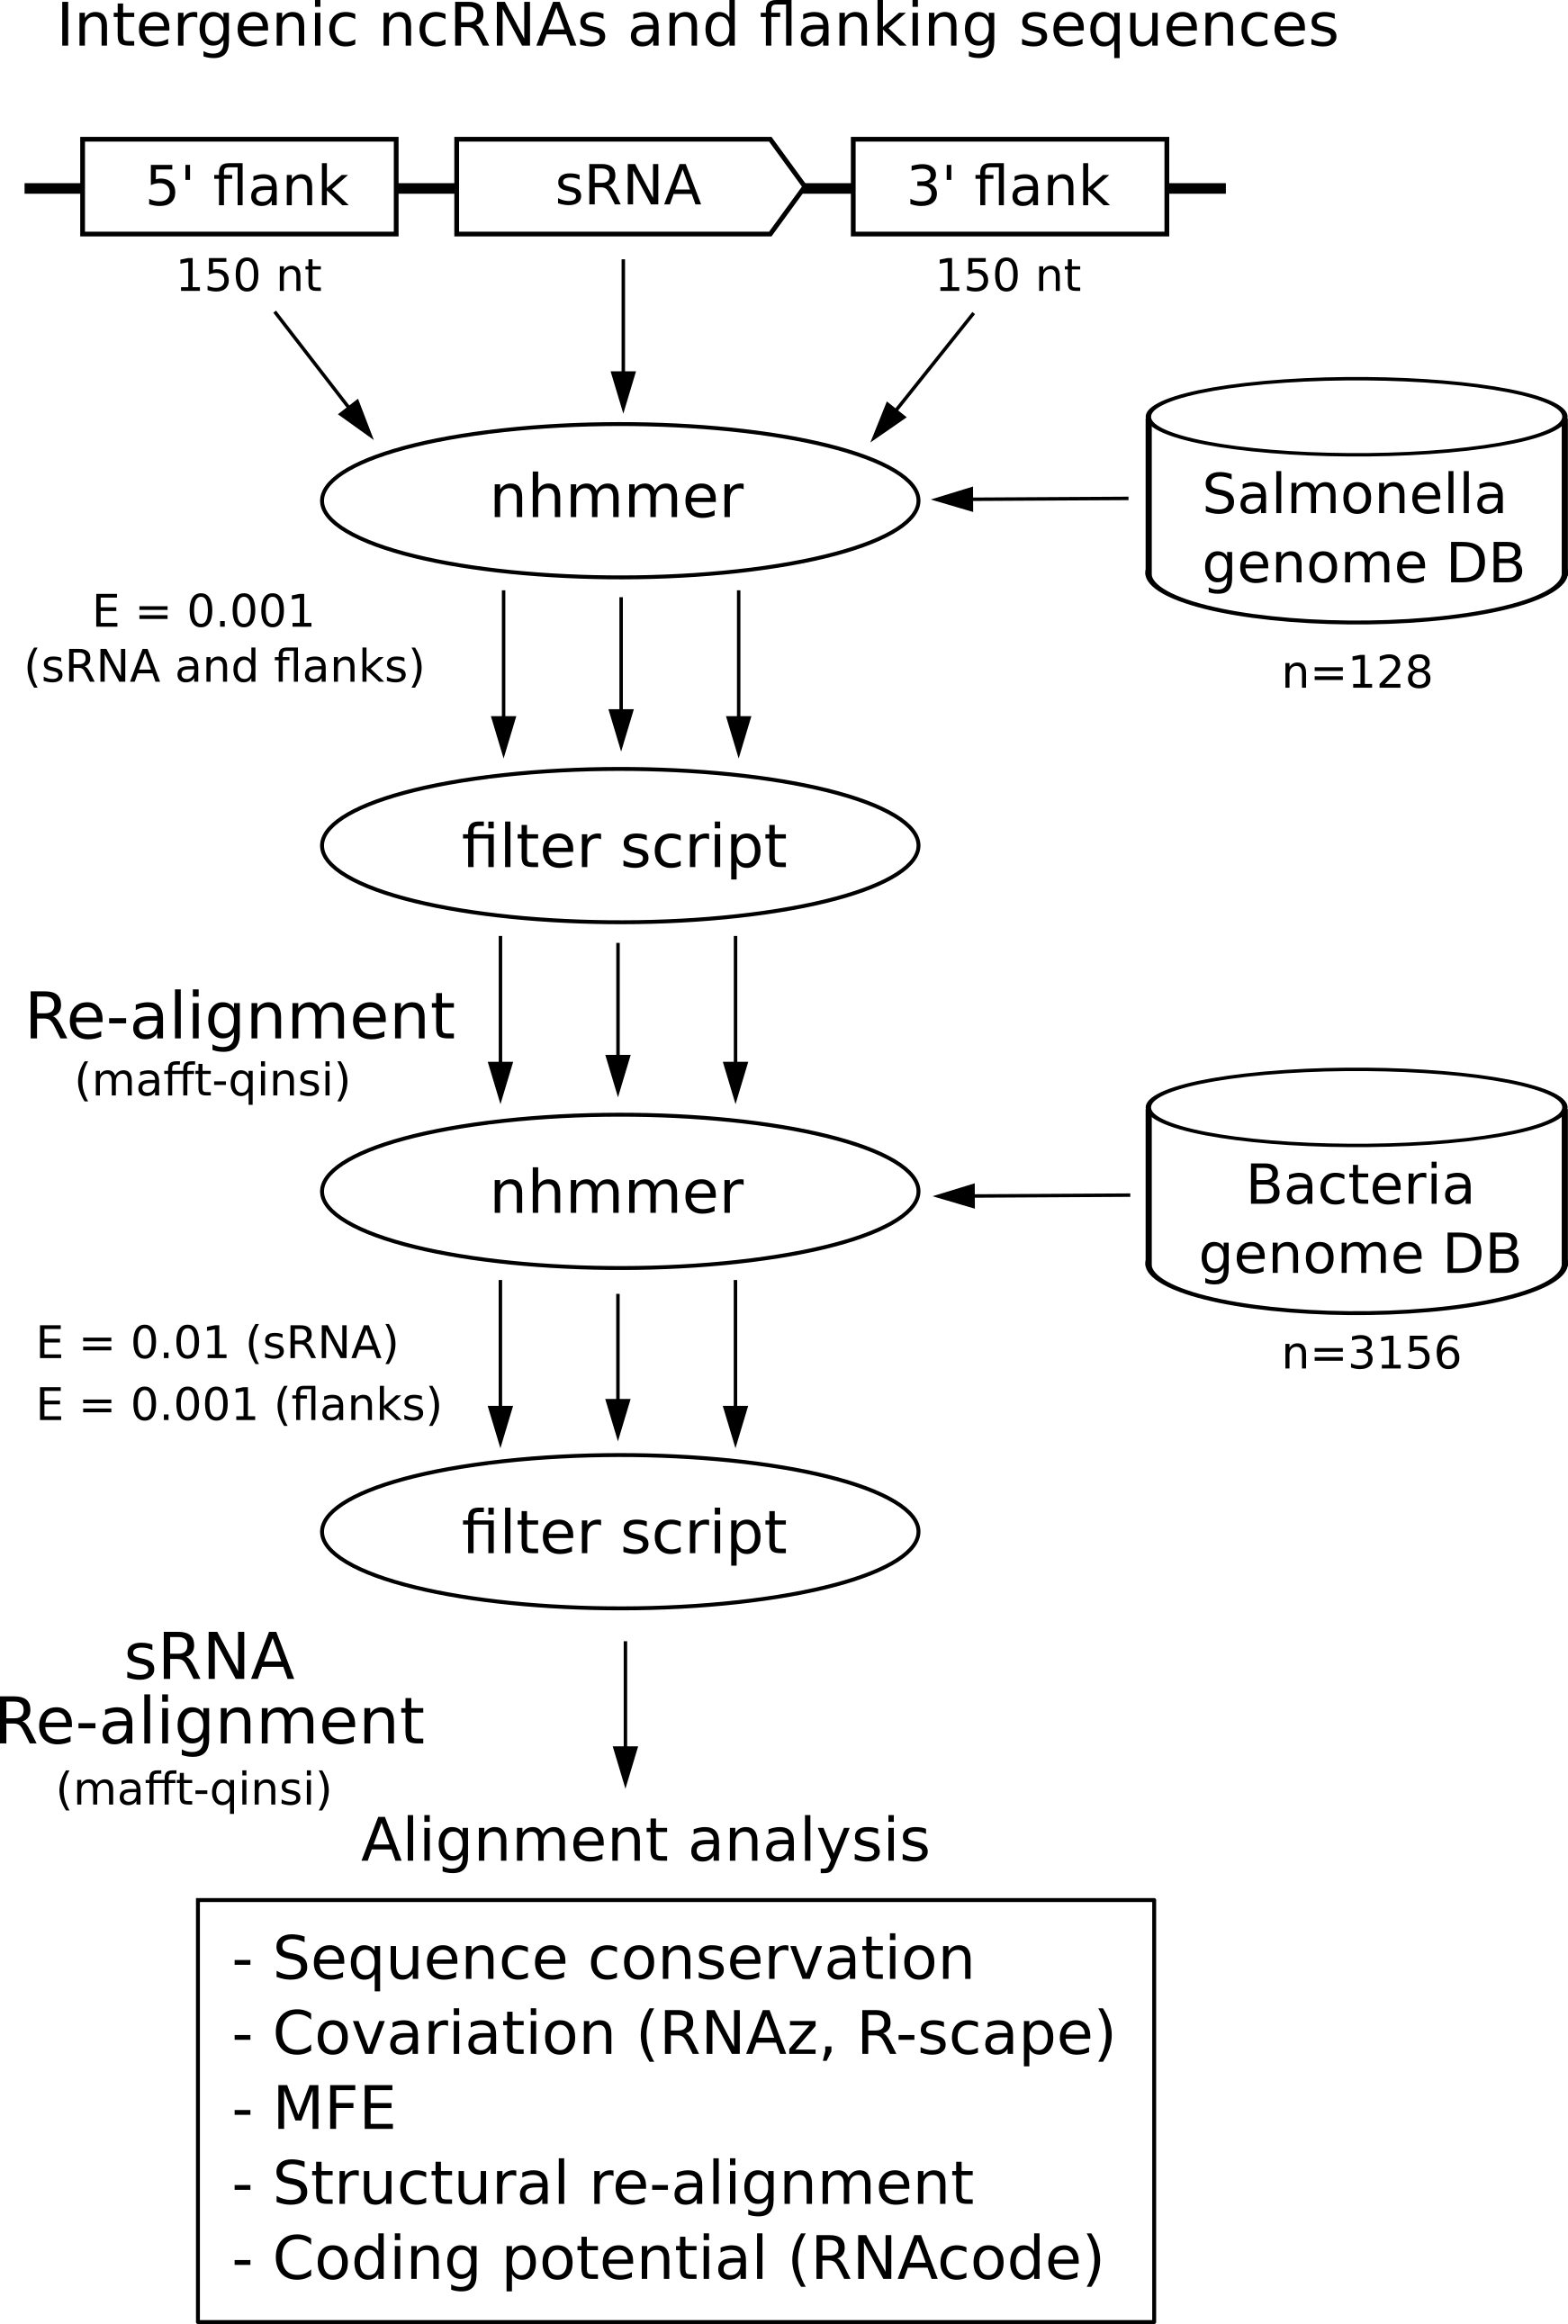
\includegraphics[scale=0.5]{sal/alternative_flowchart.png} 
\end{subfigure}
\begin{subfigure}{0.49\textwidth}
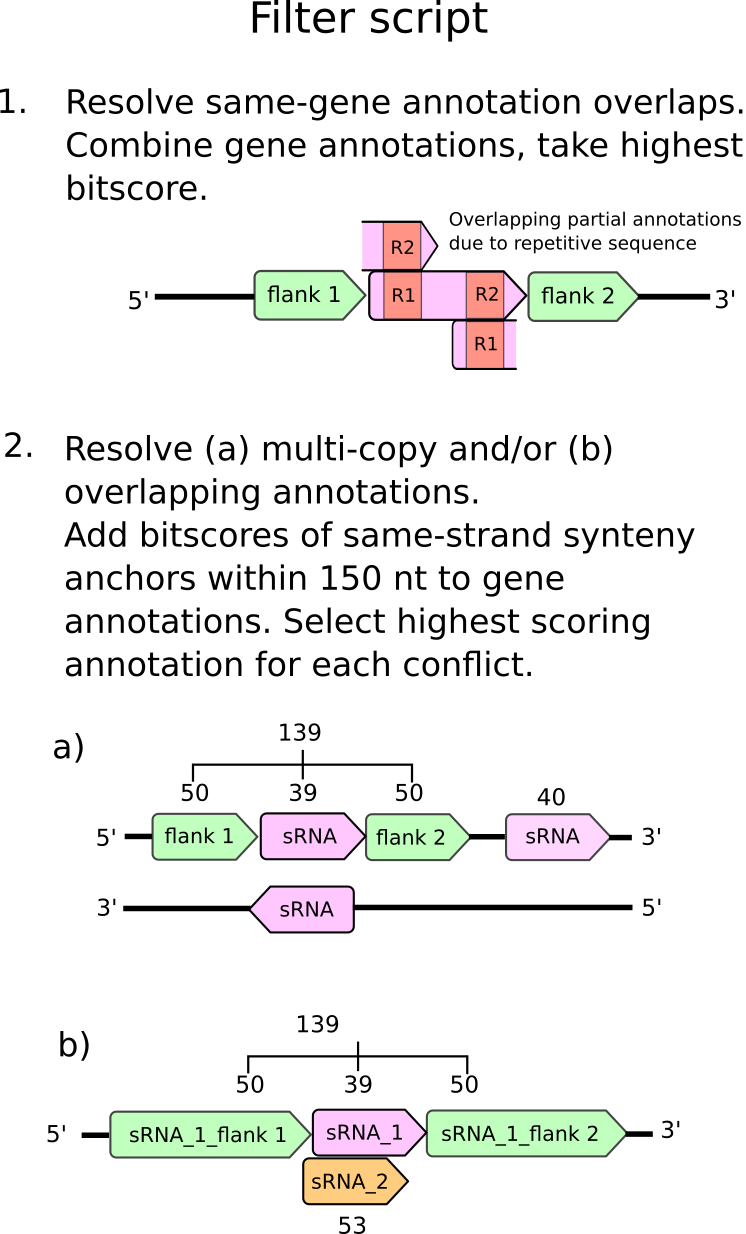
\includegraphics[scale=1.1]{sal/filter_flowchart.png}
\end{subfigure}
\caption[Flow-charts outlining the sRNA homology search pipeline, and the filtering strategy used to select homology search results]{\textbf{Left:} Flow-chart describing the homology search pipeline used. Single-sequence HMMs are used to search for homologous sequences within a genus restricted database (128 \textit{Salmonella} genomes) using \texttt{nhmmer} \citep{Wheeler2013-qxxw}. A stringent E-value threshold of 0.001 is used for this step to improve annotation accuracy and generate a trusted multiple sequence alignment. A filtering script is then used to resolve multi-copy and overlapping annotations. Multiple sequence alignments for both the sRNA and flanking sequences are generated using \texttt{mafft-qinsi} \citep{Katoh2013-wd}. New HMMs were built from each alignment and used in a second \texttt{nhmmer} homology search over the entire bacterial genome database. For this search, the E-value threshold is increased to 0.01 for sRNA genes to capture more divergent sequences. Results are filtered and used to generate final alignments. Alignments are ranked by conservation, structural stability (\texttt{RNAalifold} minimum free energy prediction), and covarying base pairs. \textbf{Right:} Filtering strategy for resolving multi-copy and overlapping ncRNA annotations. \textbf{(1)} Partial overlapping annotations of the same gene are combined. An example shows an sRNA with partial annotations around repeat regions. \textbf{(2)} For \textbf{(a)} multi-copy and \textbf{(b)} overlapping annotations, the bit-scores of each annotation and any correctly oriented synteny anchors within 150 nt are summed. The annotation with the highest bit-score is then chosen.}
\label{fig:pipeline_flowchart}
\end{figure}
\newpage
\subsection{Predicting sRNA evolutionary origins}

To predict the evolutionary origin of the genes, a database of 317,498 proteins was created from three upstream and three downstream proteins for each sRNA annotation, based on EMBL gene annotations. These proteins were functionally annotated with \texttt{eggnog-mapper} \citep{Huerta-Cepas2017-mp} using the eggNOG bactNOG HMMs \citep{Powell2012-of}. The resulting 1,444 eggNOG functional descriptions were used to estimate if proteins were part of a mobile genetic element (MGE), such as transposons (e.g transposases and integrases) or phages (e.g integrases, capsid and tail proteins). Protein descriptions from the eggnog annotations were manually binned into ‘MGE’ (n=55, list provided in Table \ref{tab:manual_MGE_terms}) and ‘non-MGE’ (n=1089).

Individual sRNAs were manually classified as "horizontally" or "vertically" inherited based on several lines of evidence. First, sRNAs were classed as candidate horizontally-acquired genes based on their proximity to annotated pathogenicity islands and prophages (annotations by \cite{Kroger2013-pg,Kroger2012-cr}). EggNOG protein descriptions were also used to indicate whether an sRNA was near, or within, a cryptic or undiscovered mobile genetic element. If any protein annotations flanking an sRNA were consistently annotated as an MGE, this was taken as a signal of horizontal gene transfer.

A sub-set of vertically-inherited sRNAs were classed as "divergence". Vertically-inherited sRNAs with inconsistent annotation across a lineage, for example otherwise conserved genes missing in a specific genus, were investigated to identify if the sRNA was missing or not annotated due to sequence divergence. The presence of closely-spaced sRNA flanking sequences was used to identify if an intergenic region known to contain an sRNA was present but not annotated due to sequence divergence.

Conservation was then used to resolve ambiguities. For example, if an sRNA was inconsistently annotated and conserved at the sequence level across the Enterobacteriaceae, this was taken as a signal of horizontal gene transfer (Figure  \ref{fig:hgt_detection}A). Unfiltered homology search results were also used to identify sRNAs with highly multi-copy annotations or partial matches to MGEs (Figure \ref{fig:hgt_detection}B). The combination of these factors was used to predict whether sRNAs were part of mobile genetic elements, or merely frequent insertion sites for MGEs. 
\begin{figure}[H]
    \centering
    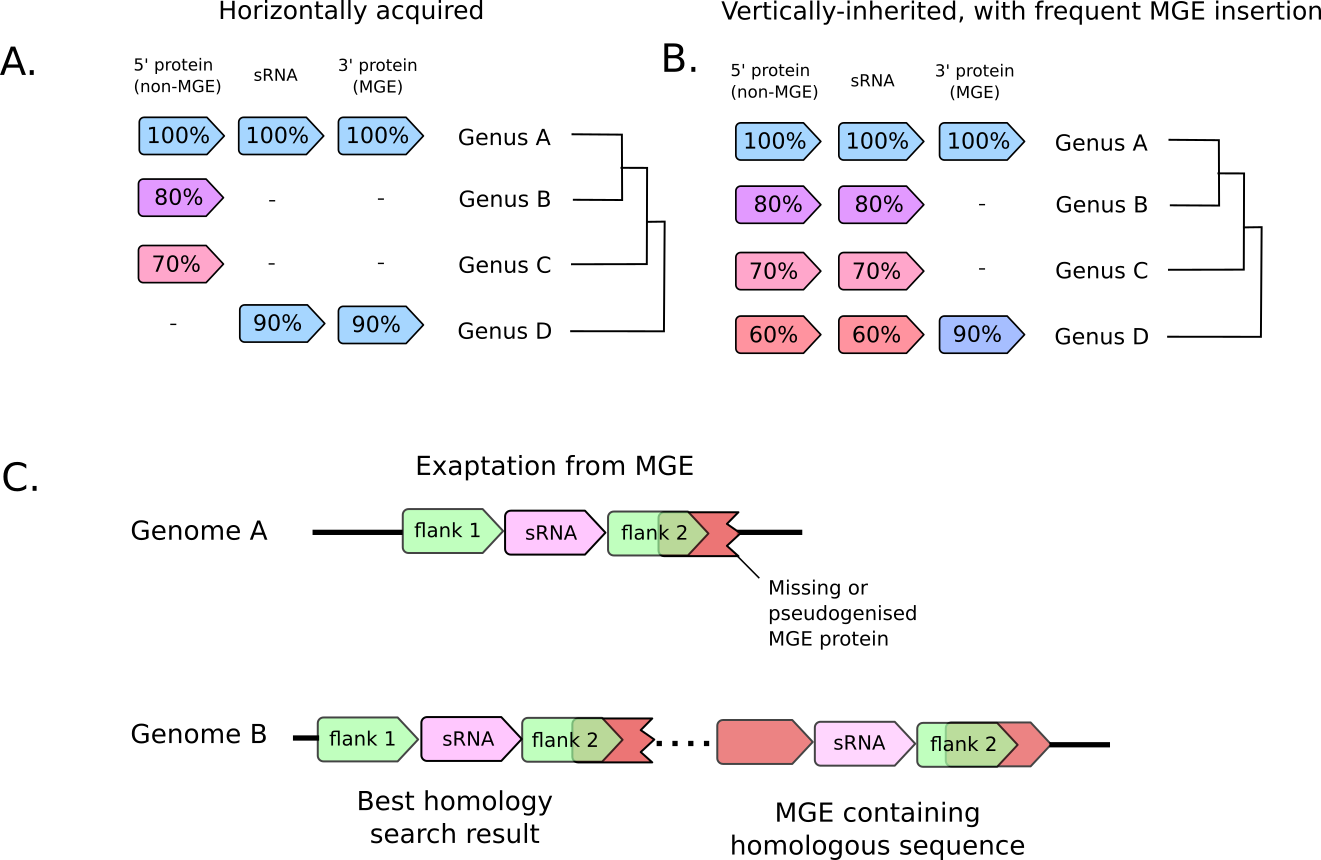
\includegraphics[scale=0.9]{sal/hgt_detection.png}
    \caption[Diagram illustrating how homology search results were used to identify sRNAs associated with MGEs]{Diagram illustrating how homology search results were used to identify sRNAs associated with MGEs. Two examples (A and B) illustrate how context can be used to identify if an sRNA associated with MGE proteins is horizontally acquired or vertically inherited. In this example, Genus A and Genus D are in the same family, but have diverged significantly. \textbf{(A)} A horizontally-acquired sRNA is present only in two distantly-related genera, and associated with an MGE protein. The sRNA also shows high sequence conservation over a large phylogenetic distance. \textbf{(B)} A vertically-inherited sRNA is consistently annotated throughout the phylogeny, and shows high sequence turnover. An MGE protein is often found near the sRNA, but is due to independent insertions within Genus A and Genus D. \textbf{(C)} An illustration showing how multi-copy homology search results can be used to identify sRNAs with homology to an sRNA contained within an MGE. An example is shown of an sRNA deposited by a previous MGE in the ancestor of Genome A and Genome B, that has been maintained after the rest of the MGE has been deleted or pseudogenised. Genome B contains both the exapted MGE sRNA locus, which is annotated by homology search, as well as an intact MGE containing a homologous sequence. Homology with this MGE can be used to infer a horizontally-acquired origin for this sRNA.}
    \label{fig:hgt_detection}
\end{figure}
\newpage
\section{Results and Discussion}
\subsection{Filtering is required to reduce false positives}

Prior to filtering many sRNAs were annotated as multi-copy (Figure \ref{fig:copy_number}), due to shared sequence features with each other, and with existing genomic elements. Some HMMs built from short sRNA sequences generated highly multi-copy homology search results, producing hundreds of annotations per genome. An extreme example of this was \textit{c0664}, which was annotated at the end of almost all coding sequences in each \textit{Salmonella} genome prior to filtering. 

\begin{figure}[H]
    \centering
        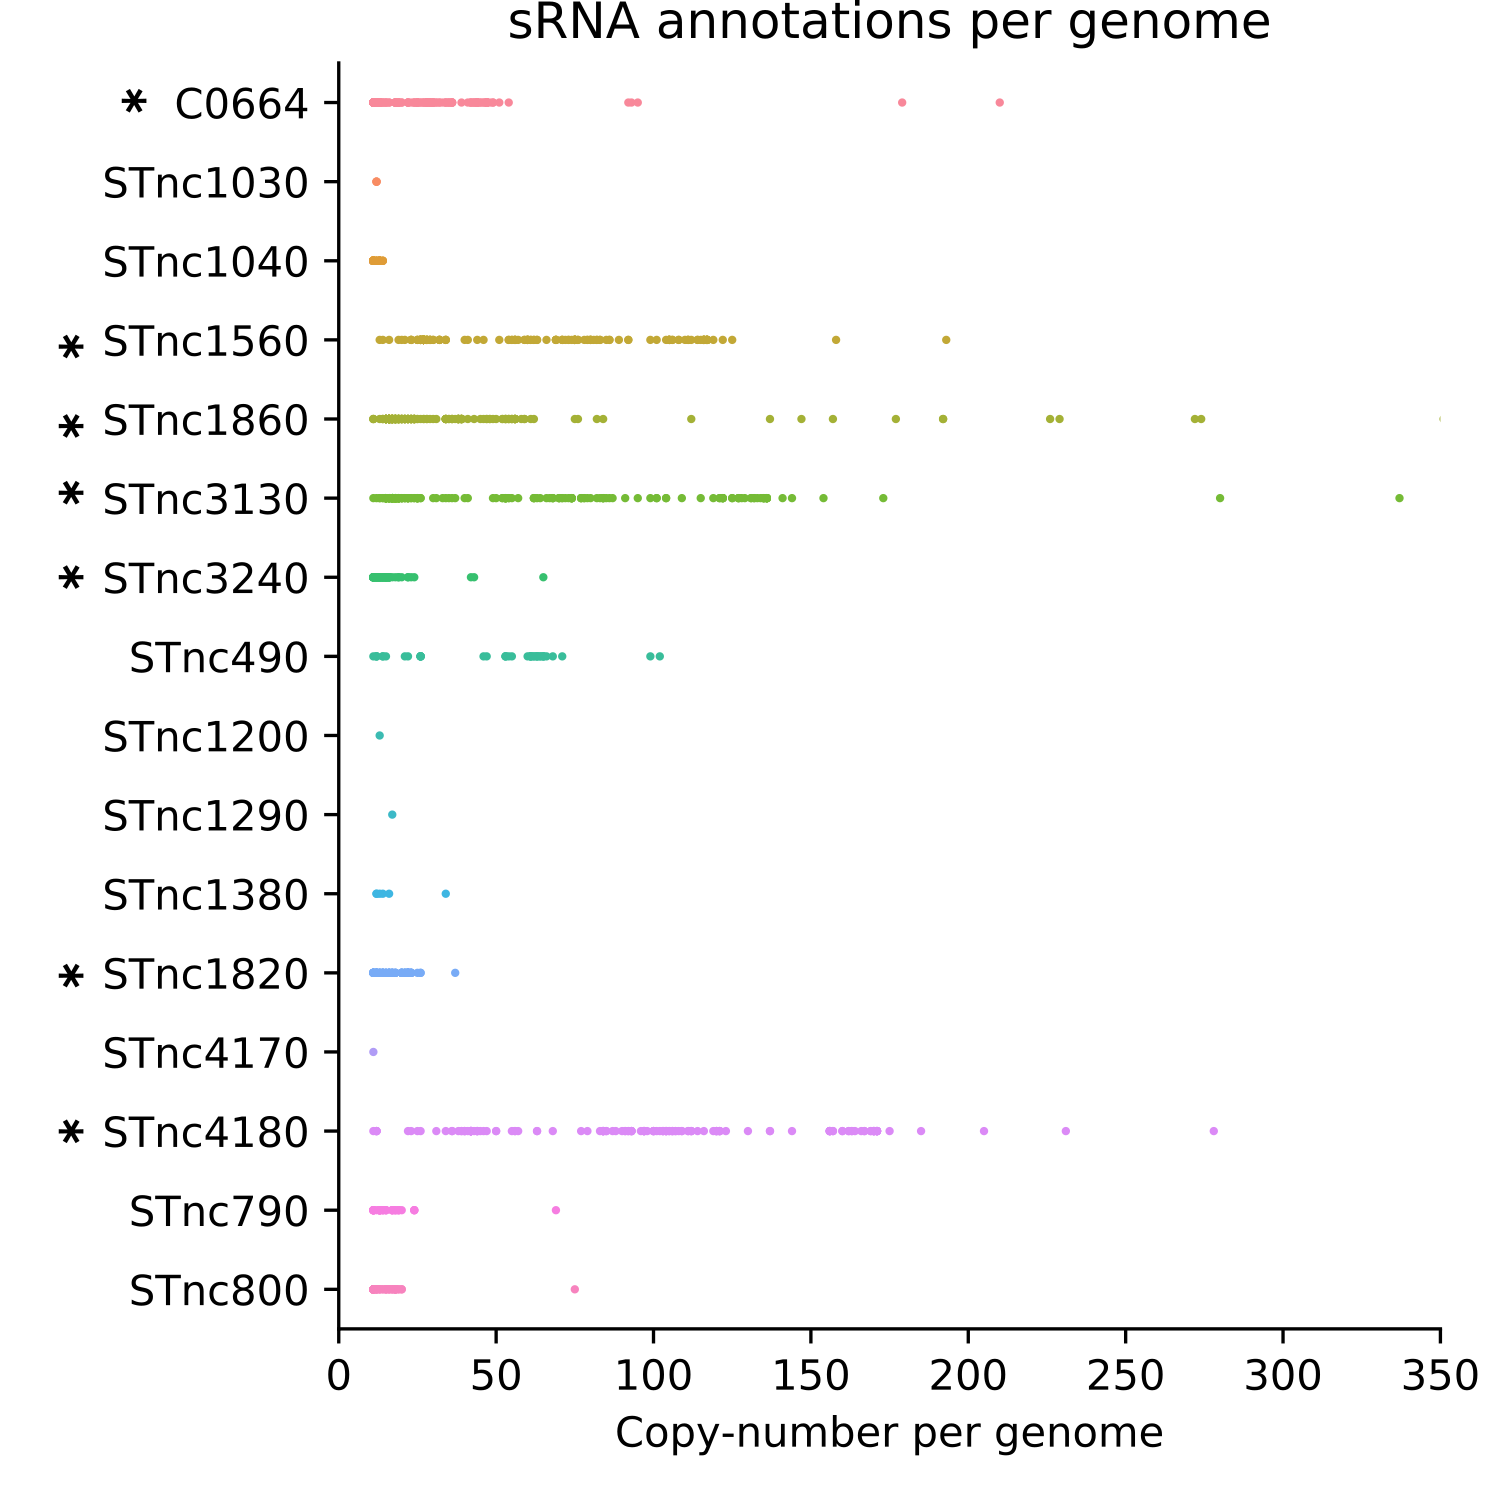
\includegraphics{sal/copy_number.png}
    \caption[Copy number per genome for multi-copy sRNAs.]{Copy number per genome for highly multi-copy sRNAs. Number of homology search results per genome prior to filtering are plotted for genes with >10 copies per genome. \textbf{*} denotes genes that were found to overlap with annotated repetitive extragenic palindromes (REPs) in \textit{E. coli} str. K12 substr. MG1655 (genome accession U00096.3) (shown in Figure \ref{fig:REP_motifs}). }
    \label{fig:copy_number}
\end{figure}
\newpage
Many of the most highly multi-copy sRNAs (\textit{c0664}, \textit{STnc1560}, \textit{STnc1820}, \textit{STnc1860}, \textit{STnc3130}, \textit{STnc3240} and \textit{STnc4180}) had annotations that overlapped with repetitive extragenic palindromic (REP) elements in \textit{E. coli} str. K12 substr. MG1655 (genome accession U00096.3). REP elements are 30-40 nt short intergenic repeats found downstream of stop codons in gammaproteobacteria, which make up \textasciitilde0.5-1\% of the \textit{E. coli} genome \citep{Stern1984-eq,Dimri1992-uf}. 

REPs can help form and stabilise hairpin loops within transcripts, and can function to regulate mRNA transcription \citep{Espeli2001-bk}, polycistronic transcript stability and decay \citep{Khemici2004-ch}, and translation \citep{Liang2015-yy}. \textit{c0664} is known to contain an REP element \citep{Hershberg2003-qxi}, and other sRNAs which overlapped with REPs had conserved REP-like imperfect palindromic sequences in predicted stem-loop secondary structures (Figure \ref{fig:copy_number}).

Short sRNAs with sequence similarity to REP elements are likely to produce false positive annotations where the REP element forms a substantial proportion of the sRNA gene. For example, \textit{c0664} has previously been reported at over 40 copies per genome in a BLAST-based analysis \citep{Skippington2012-iv}. Further work is needed to confirm if these sRNAs are REP elements, and if highly multi-copy sRNAs that are annotated at the 3$\textprime$ end of protein-coding sequences may contain novel REP motifs. 

Other structured sRNAs containing palindromic sequences produced multiple partial intra-gene annotations on each strand, and models for recent paralogues such as \textit{glmZ} and \textit{glmY} converged on each other prior to the implementation of synteny anchor-based filtering. Filtered annotations generated in this project closely matched those from the original \textit{Salmonella} Typhimurium ST4/74 sRNAs, and closely overlapped (0-64 nt difference in gene boundaries) with known homologues annotated in \textit{E. coli} K12, and a set of sRNA annotations collected from literature by \cite{Richter2012-uuuuiu} (Figure \ref{fig:start_finish}), indicating that filtering with synteny anchors removed the majority of false positives for intergenic sRNAs.


\begin{figure}[H]
\centering
        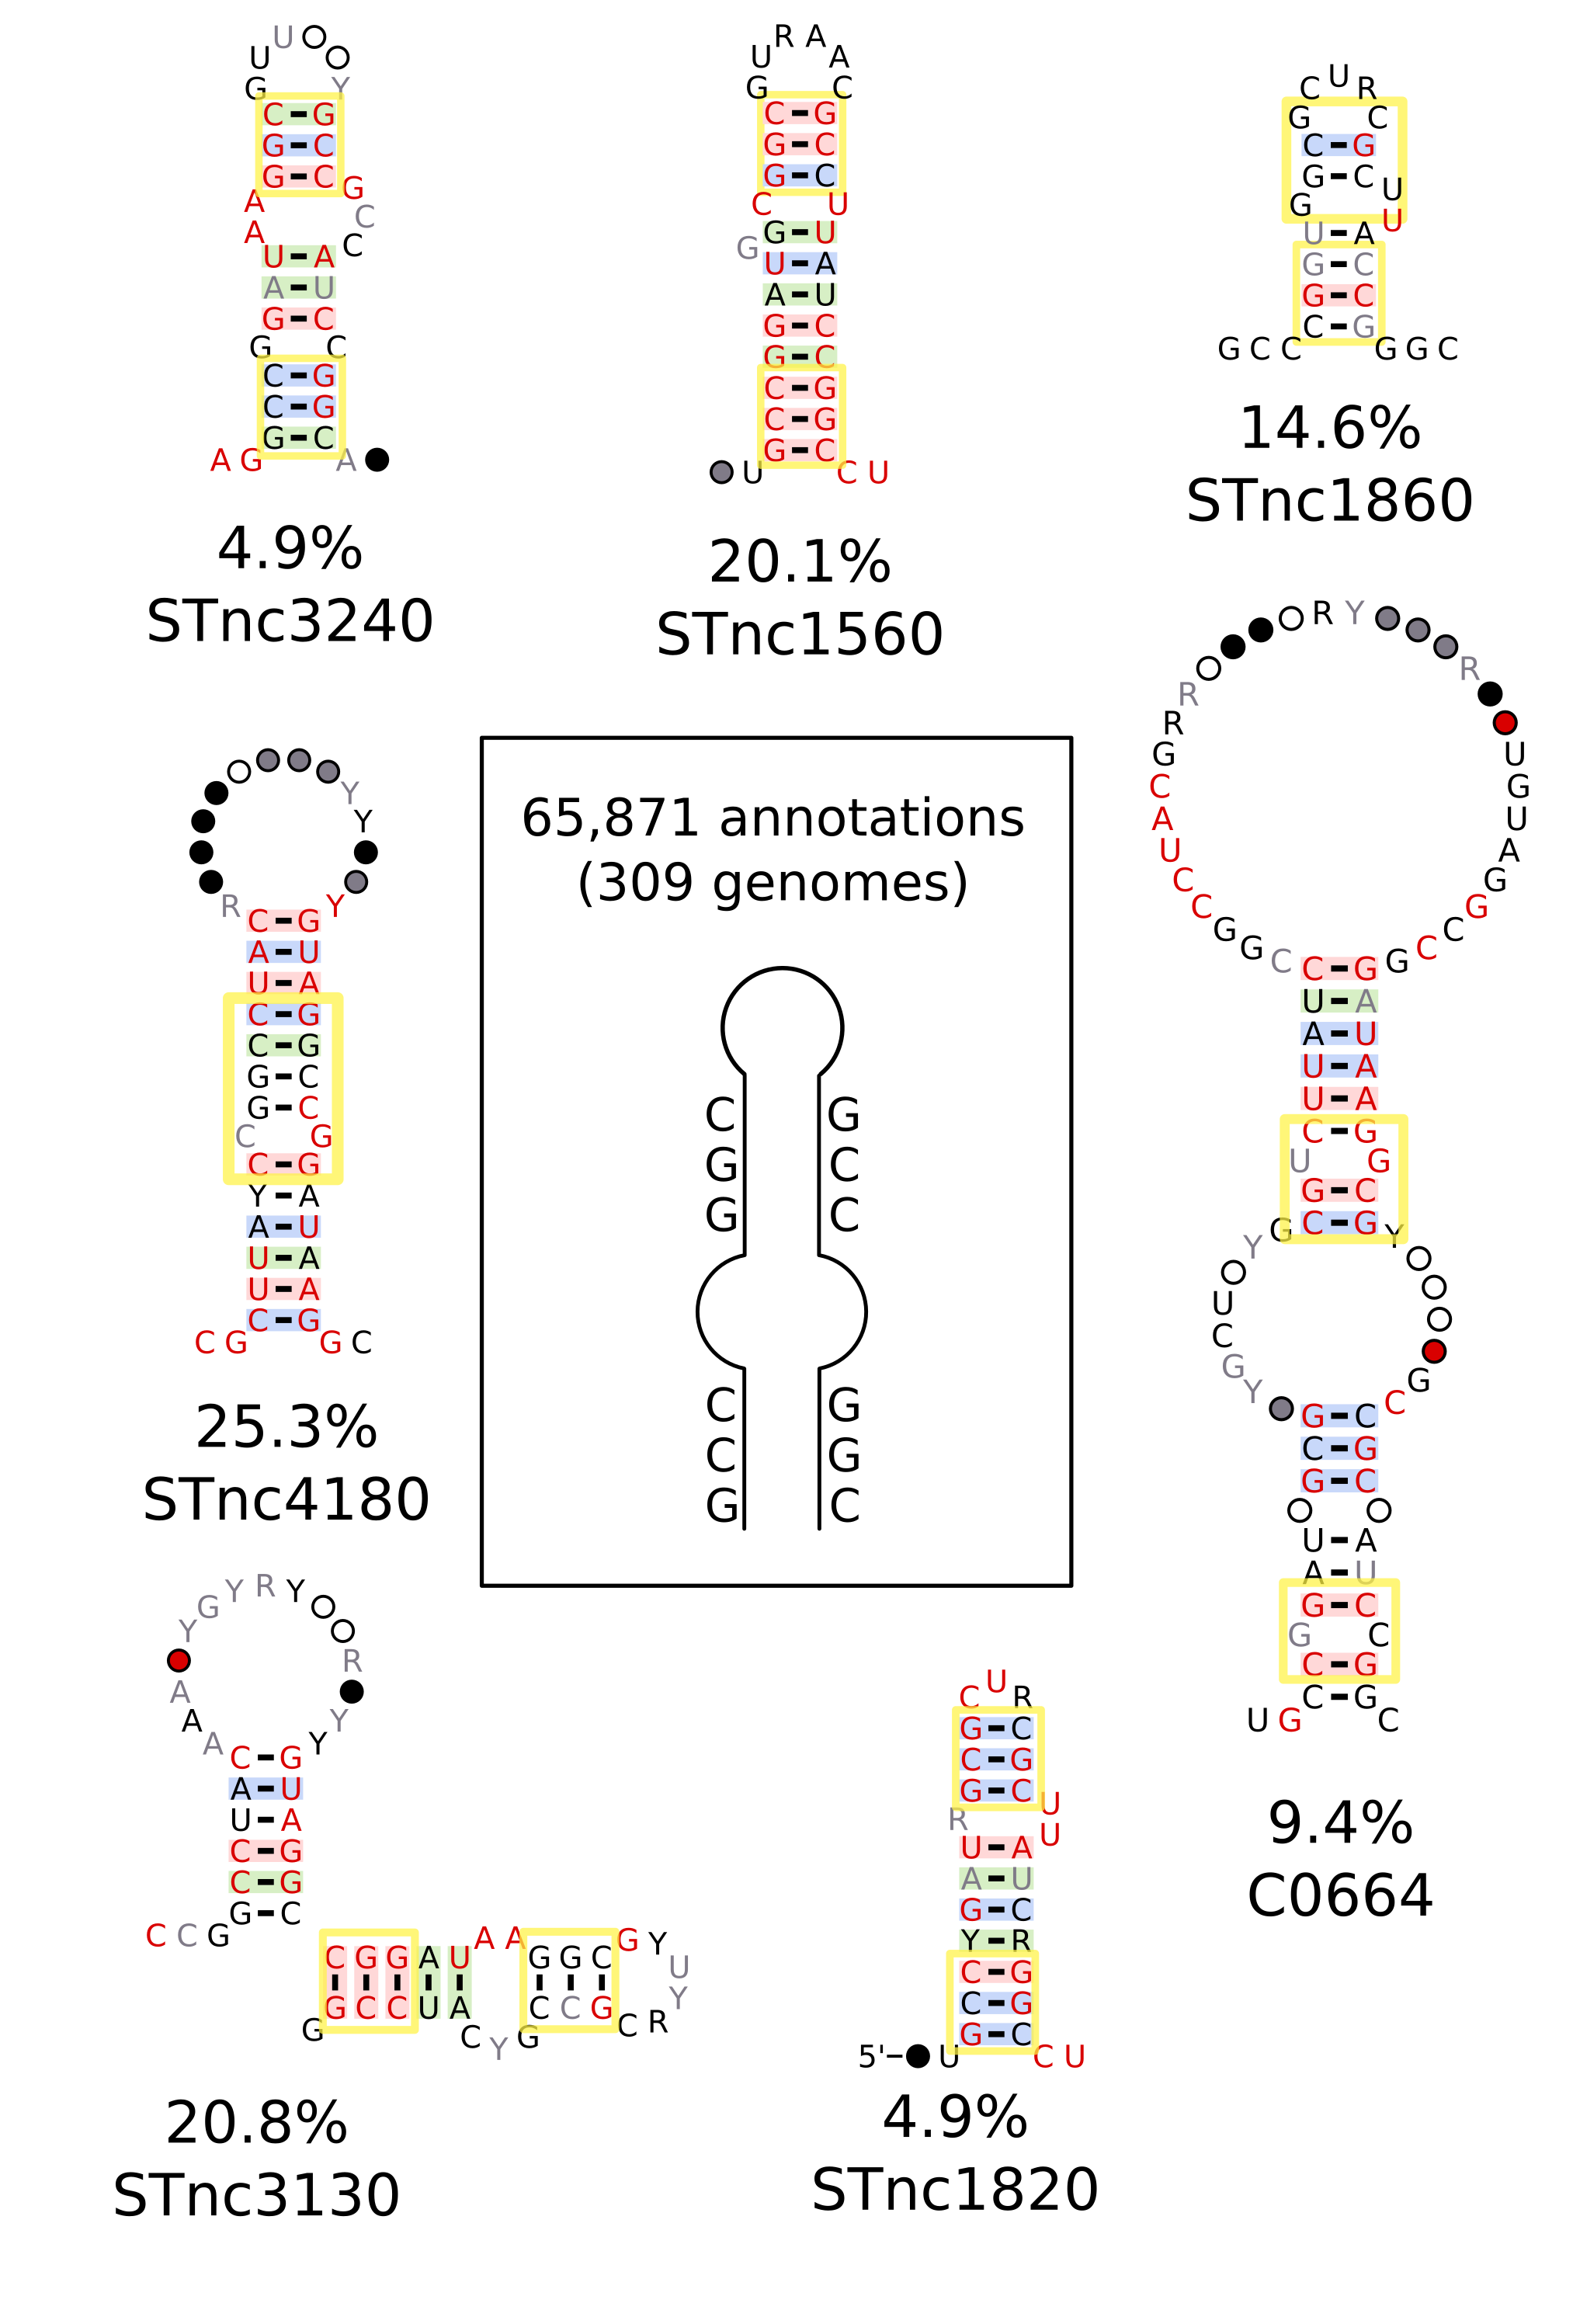
\includegraphics[scale=0.75]{sal/REP_motifs.png}
    \caption[Predicted consensus secondary structures for sRNAs with sequence similarity to REPs]{Predicted consensus secondary structures for sRNAs with sequence similarity to annotated REPs in  \textit{E. coli} str. K12 substr. MG1655 (based on annotation overlap with REP annotations for U00096.3 on NCBI). A total of 65,871 annotations of these seven genes were generated during homology search, the proportions of which are shown for each sRNA. A representative \textit{E. coli} REP motif \citep{Tobes2006-kd} within a stem-loop structure is shown. REP-like motifs are highlighted on the structures in yellow.}
    \label{fig:REP_motifs}
\end{figure}
\newpage

\begin{figure}[H]
    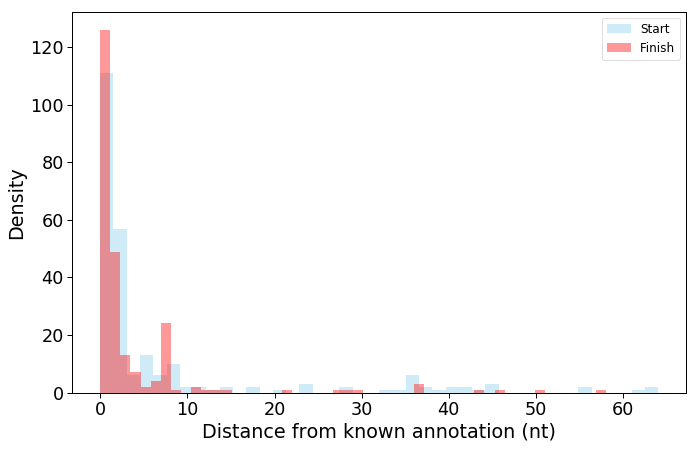
\includegraphics[scale=0.6]{sal/start_finish.png}    
    \caption[Comparison of sRNA annotations by \cite{Richter2012-uuuuiu} and from this study]{Comparison of sRNA annotations by \cite{Richter2012-uuuuiu} and from this study (n=243). Gene boundary differences (distance from start and stop) in genomes and genes present in both data-sets are plotted as a histogram, showing that these annotations closely overlap. The annotations had no differences in orientation.}
    \label{fig:start_finish}
\end{figure}

\subsection{Recent acquisition and sequence divergence of \textit{Salmonella} sRNAs }

The sequence conservation of homology search results across the Enterobacteriaceae, visualised as a heatmap in Figures \ref{fig:sal_heatmap}B and \ref{fig:sal_heatmap2}B, broadly mirrors previous observations that the majority of sRNAs both evolve rapidly and are restricted to a genus or species \citep{Gomez-Lozano2015-yx,Gottesman2011-vx,Skippington2012-iv}. 
The conservation of sequences flanking sRNAs, most of which overlapped with coding sequences, were used to estimate if sRNAs were limited to a lineage and not approaching the lower bound of sequence alignment due to sequence variation. The majority of vertically-inherited sRNAs had similar phylogenetic distributions to at least one flanking sequences, which were limited to a sub-lineage of the Enterobacteriaceae. 

The rate of sequence turnover, defined here as observable change in nucleotide sequence over time, appears to be proportional to the age of sRNA genes investigated in this study. High rates of sequence divergence (a change from 100\% to \textasciitilde50\% sequence identity) could be seen between sRNAs limited to the  \textit{Salmonella}-\textit{Escherichia} lineage, as between larger phylogenetic distances such as between \textit{Salmonella} and \textit{Yersinia} sequences (Figure \ref{fig:PID_plots}). 

Only 9 intergenic \textit{Salmonella} sRNAs were found to be conserved across the Enterobacteriaceae, all of which except \textit{sdsR}, \textit{spf}, \textit{sroG} and \textit{STnc700} were family-specific. Several other sRNAs were highly conserved in all genera except in the obligate plant pathogens \textit{Edwardsiella}, \textit{Xehnorhabdus} and \textit{Pectobacterium}. With the exception of \textit{spf}, all highly conserved sRNA genes exhibited high sequence divergence, with homologous sequences in the genera most distantly related to \textit{Salmonella} having only \textasciitilde40\% sequence similarity to their \textit{Salmonella} counterparts. \textit{spf} was found to be highly conserved throughout the Enterobacteriaceae, and had the least amount of sequence variation, with the lowest average percentage sequence identity of 93\% in \textit{Dickeya}. 

\begin{figure}[H]
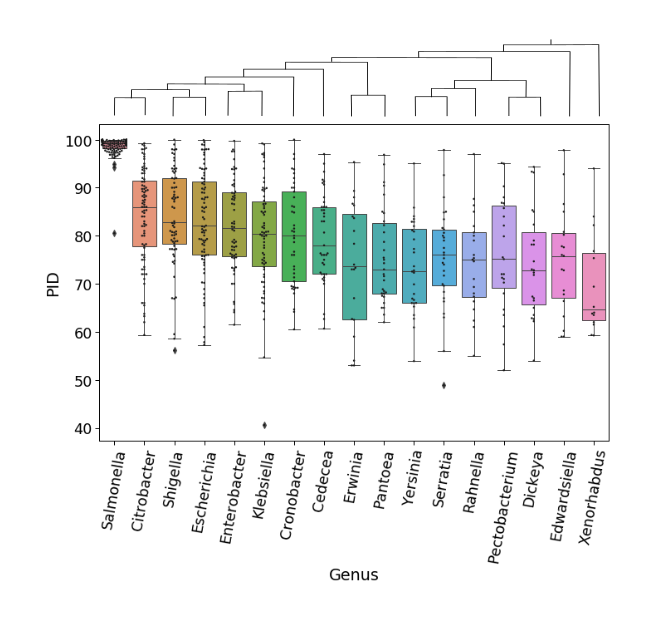
\includegraphics[scale=1.7]{sal/genus_PID_with_tree.png} 
\caption[Boxplots showing sRNA sequence variation within different genera]{Boxplots showing sRNA sequence variation within different genera. PID (percentage sequence identity) relative to the \textit{S.} Typhimurium ST4/74 sequence measurements for vertically-inherited sRNA annotations from the homology search are shown, separated by genus. Genera are ordered by phylogenetic distance from \textit{Salmonella}, and approximate phylogenetic relationships are shown above the plot.}
    \label{fig:PID_plots}
\end{figure}

In total 74/200 sRNAs were only found within \textit{Salmonella} (shown in Figure \ref{fig:sal_heatmap}), and overall the majority of sRNAs were restricted to the \textit{Salmonella}-\textit{Escherichia} lineage, and showed rapid within-lineage divergence. Although many sRNAs in this data-set have yet to be functionally characterised, there does appear to be a correlation between the specificity of function and conservation of an sRNA gene. 

Highly conserved sRNAs are known to be involved in essential cellular processes, such as the 6S RNA, which is involved in the regulation of transcription \citep{Wassarman2007-dxx}, or well integrated into large regulons, such as the CsrB sRNA, which sequesters the highly conserved carbon storage regulator CsrA \citep{Babitzke2007-bb}. Conversely, sequence and gene conservation was reduced in \textit{Erwinia, Pectobacterium, Pantoea, Dickeya}, and \textit{Xenorhabdus}, which are obligate plant pathogens that have substantial genomic and phenotypic differences other genera in the family, which are animal gut pathogens and commensals \citep{Toth2006-xt}. 
%structure conservation - HGT-acquired and poorly conserved sRNAs have lower MFE secondary structure prodictions. Few vertically inherited Salmonella-specific genes show signs of secondary structure

The variation of function and sequence diversity decreases for sRNA genes are more widely conserved throughout the Enterobacteriaceae. Genus or lineage-specific sRNAs often contribute to niche adaption, and show more sequence variation across small phylogenetic distances, indicating that selection pressures and essentiality of the sRNA regulon restricts sequence diversity. 

\textit{S.} Typhimurium sRNAs conserved in the \textit{Salmonella}-\textit{Escherichia} lineage are often involved in niche-specific stress responses that promote survival \textit{in vivo}. Two characterised examples are RydC, which suppresses biofilm formation and cell adhesion during nutrient availability \citep{Bordeau2014-ul}, and MgrR, which is expressed in response to low Mg\textsuperscript{2+} concentrations conditions found \textit{in vivo}, and regulates the formation of external lipopolysaccharides as part of a strategy to avoid recognition by the host immune system \citep{Moon2009-dd,Moon2013-uu}. Both of these sRNAs show sequence divergence (\textasciitilde80-85\% sequence identity in \textit{E. coli} relative to \textit{Salmonella}) and have been observed to have additional specific functions unique to \textit{Salmonella} or \textit{Escherichia}. Similarly, many \textit{Salmonella enterica}-specific sRNAs have been found to function in survival and virulence in highly specific infection conditions \citep{Colgan2016-hk,Barquist2013-ii}. Two \textit{Salmonella}-specific sRNAs, \textit{STnc2050} and \textit{STnc3750}, also have varied expression across different strains of \textit{S.} Typhimurium \citep{Canals2019-yv}.
\begin{figure}[H]
    \centering
    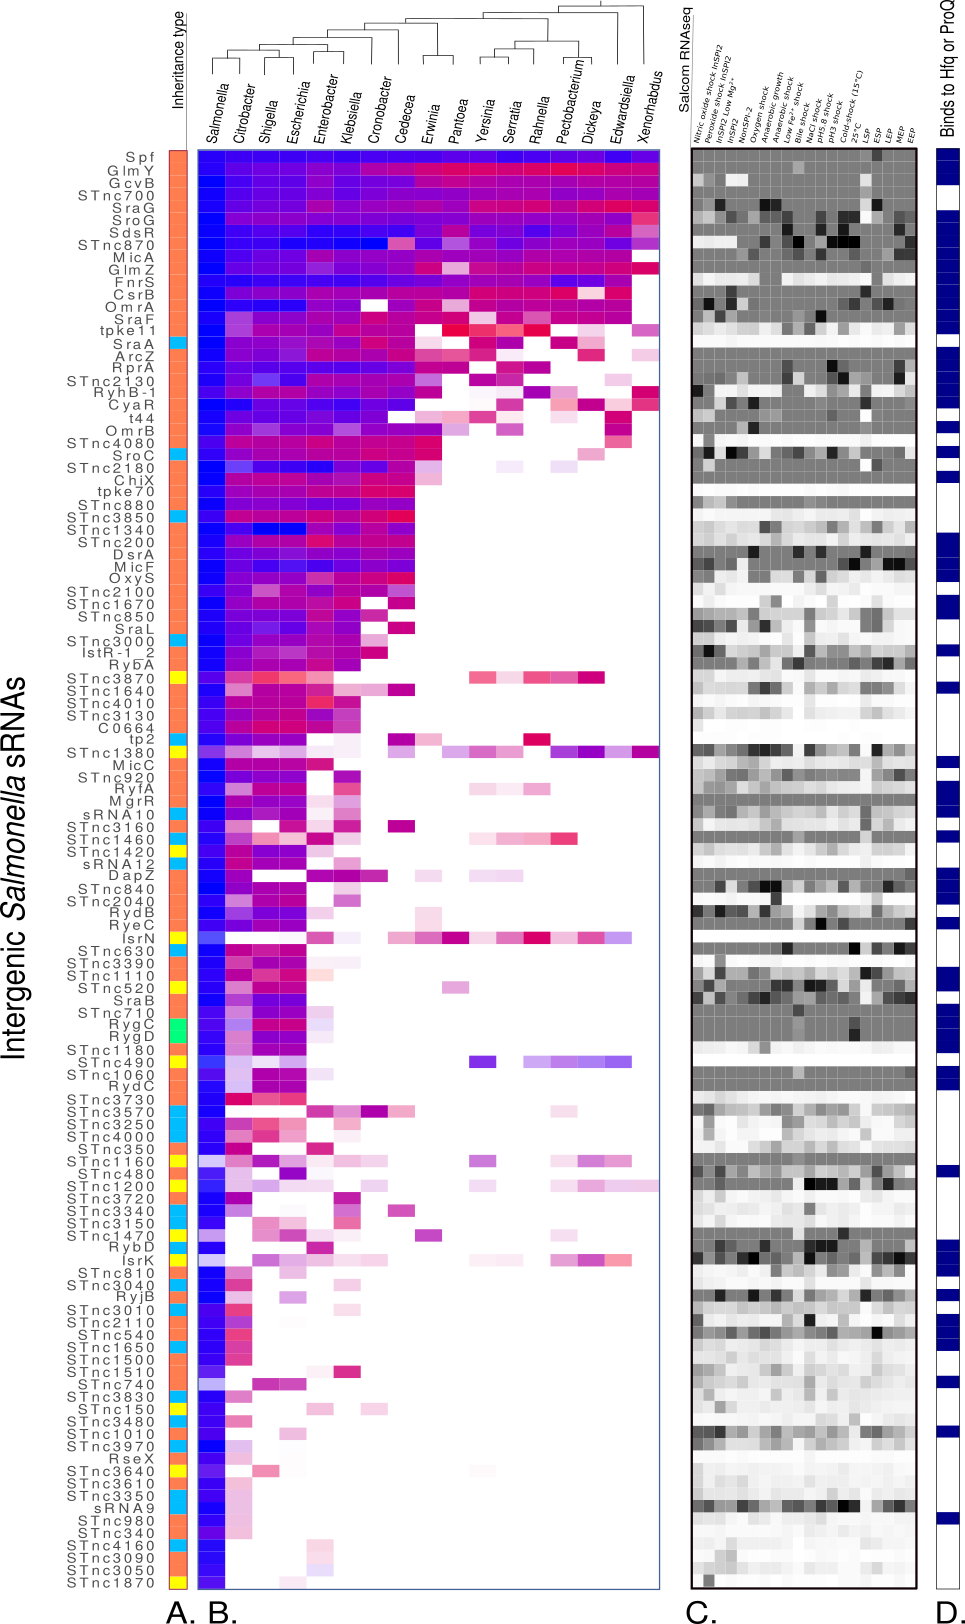
\includegraphics{sal/heatmap_split_2.png}
    \caption{Full figure caption is provided in Figure \ref{fig:sal_heatmap}}
    \label{fig:sal_heatmap2}
\end{figure}
\newpage
\newpage
\begin{figure}[H]
    \centering
    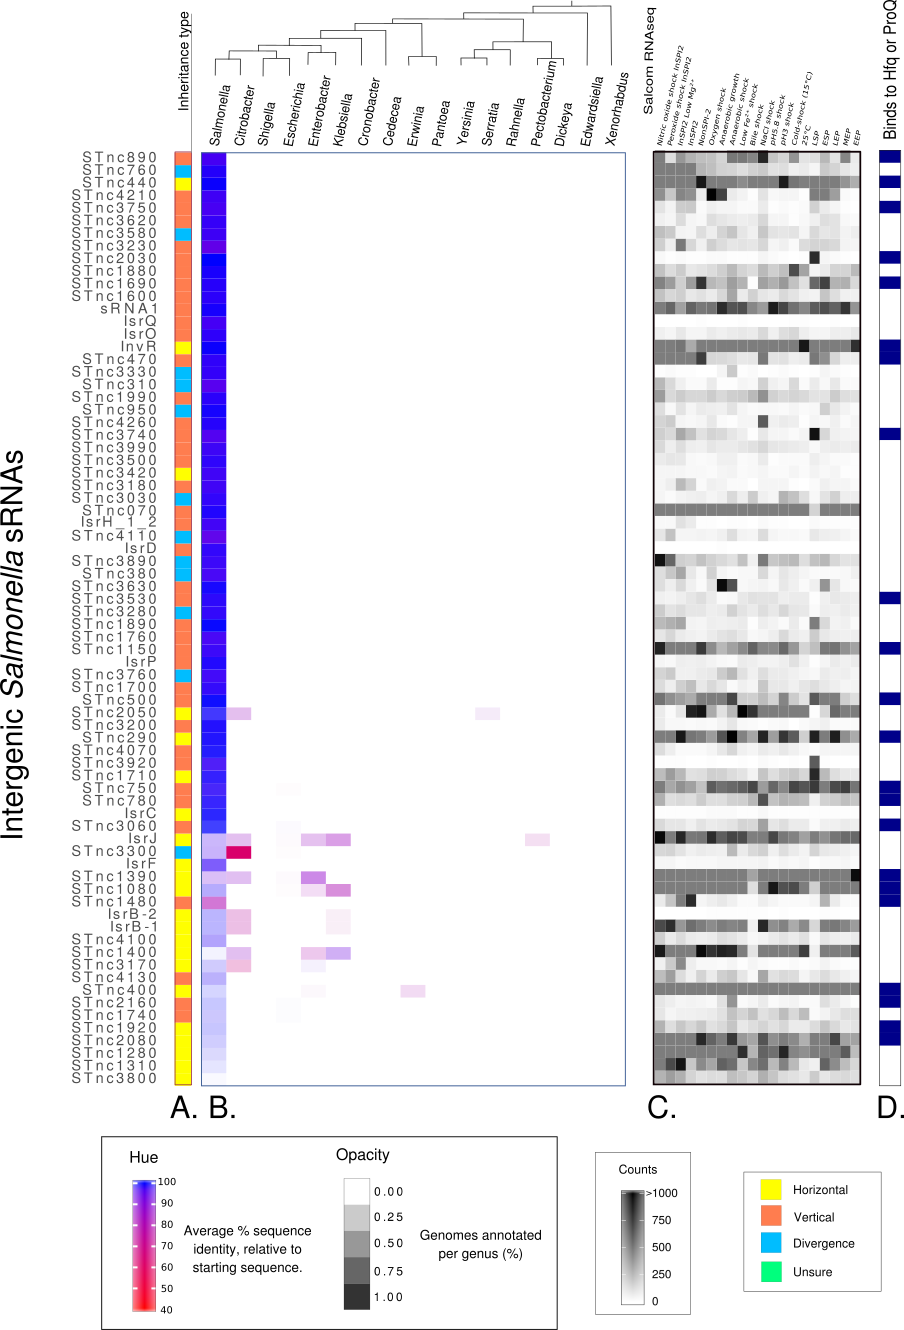
\includegraphics{sal/heatmap_part1.png}
    \caption[Conservation, expression and predicted evolutionary origins of \textit{Salmonella} sRNA genes]{Conservation, expression and predicted evolutionary origins of \textit{Salmonella} sRNA genes. \textbf{(A)} Predicted inheritance type. \textbf{Horizontal}$:$ Acquired through horizontal gene transfer. \textbf{Divergence}$:$ The locus containing an sRNA is conserved, but sRNA sequence similarity is too low for it to be annotated \textit{via} homology search. \textbf{Vertical}$:$ No signals of horizontal gene transfer. \textbf{(B)} Heatmap showing the annotation range and sequence conservation of intergenic \textit{Salmonella} sRNA genes in Enterobacteriaceae genomes. Sequence conservation is shown as a colour gradient from blue (100\%) to red (40\%), representing genus average percent sequence identity based on alignment of homology search results to the corresponding \textit{Salmonella} Typhimurium ST4/74 sequence. Gene conservation is shown as a change in opacity, represented by the percentage of genomes with an annotation within that genus. Genes are ordered based on overall conservation. Additional panels show information for the same genes from different data-sets. \textbf{(C)} RNA-seq counts (Transcripts per million) across 22 infection-relevant growth conditions (capped at 1000 TPM) from \cite{Kroger2013-pg}. \textbf{(D)} sRNA binds to Hfq \citep{Holmqvist2016-hj} or ProQ \citep{Smirnov2016-yt}.}
    \label{fig:sal_heatmap}
\end{figure}
\newpage

\subsection{Sequence composition and turnover can hamper annotation}

Thirty-six sRNAs were undetectable by homology search due to sequence divergence, large insertions or deletions. An example of this is the \textit{tp2} gene located within a pyruvate metabolic locus, which is highly conserved across the Enterobacteriaceae. The \textit{tp2} synteny anchors, consisting of the 3$\textprime$ and 5$\textprime$ ends of the proteins adjacent to \textit{tp2} (a pyruvate dehydrogenase sub-unit, and a pyruvate dehydrogenase regulator) were found in same orientation and approximate distance apart throughout the family. Alignment of the intergenic region between the \textit{tp2} synteny anchors in \textit{Klebsiella pneumoniae} (NCBI accession: CP008929) to the \textit{Salmonella} Typhimurium ST4/74 \textit{tp2} sequence identified an 18 nt insertion in \textit{Klebsiella pneumoniae}, accounting for a large proportion of the sequence (Figure \ref{fig:tp2_sroc_alignment}).

Large changes in sequence length have been previously observed in Enterobacteriaceae sRNAs. The MicF RNA, which is also in a conserved locus, has been previously annotated in \textit{Yersinia} using synteny information and BLAST searches for \textit{micF} flanking sequences from \textit{E. coli}. \citep{Delihas2003-bp}. Comparison of the \textit{micF} sequences from \textit{E. coli}, \textit{Yersinia} and \textit{Serratia} sp. found indels of 6--12 nt across the RNA and promoter region, in addition to high sequence variation, despite the MicF RNAs from these species having conserved functions. 

Synteny has also been used to annotate SgrS, an sRNA containing a protein-coding region, which can vary from in length by over 300 nt, by using the presence of a conserved flanking gene \textit{sgrR} to identify the correct intergenic region \citep{Horler2009-va}.  

The sequence composition of certain sRNAs made annotation with HMMs difficult. The RseX sRNA, which has been experimentally confirmed in \textit{E. coli} \citep{Douchin2006-dv}, was not found outside of \textit{Salmonella} in this study. Although the \textit{Salmonella} and \textit{E. coli} \textit{rseX} sequences share 70\% sequence identity, the short length and biased composition of single-nucleotide repeats in both sequences led to the results being filtered by the composition bias filter in \texttt{nhmmer}. Results returned for \textit{E. coli} \textit{rseX} with and without (\texttt{--nobias}) this filter generated annotations with bit-scores below the detection threshold of the pipeline.

\begin{figure}[H]
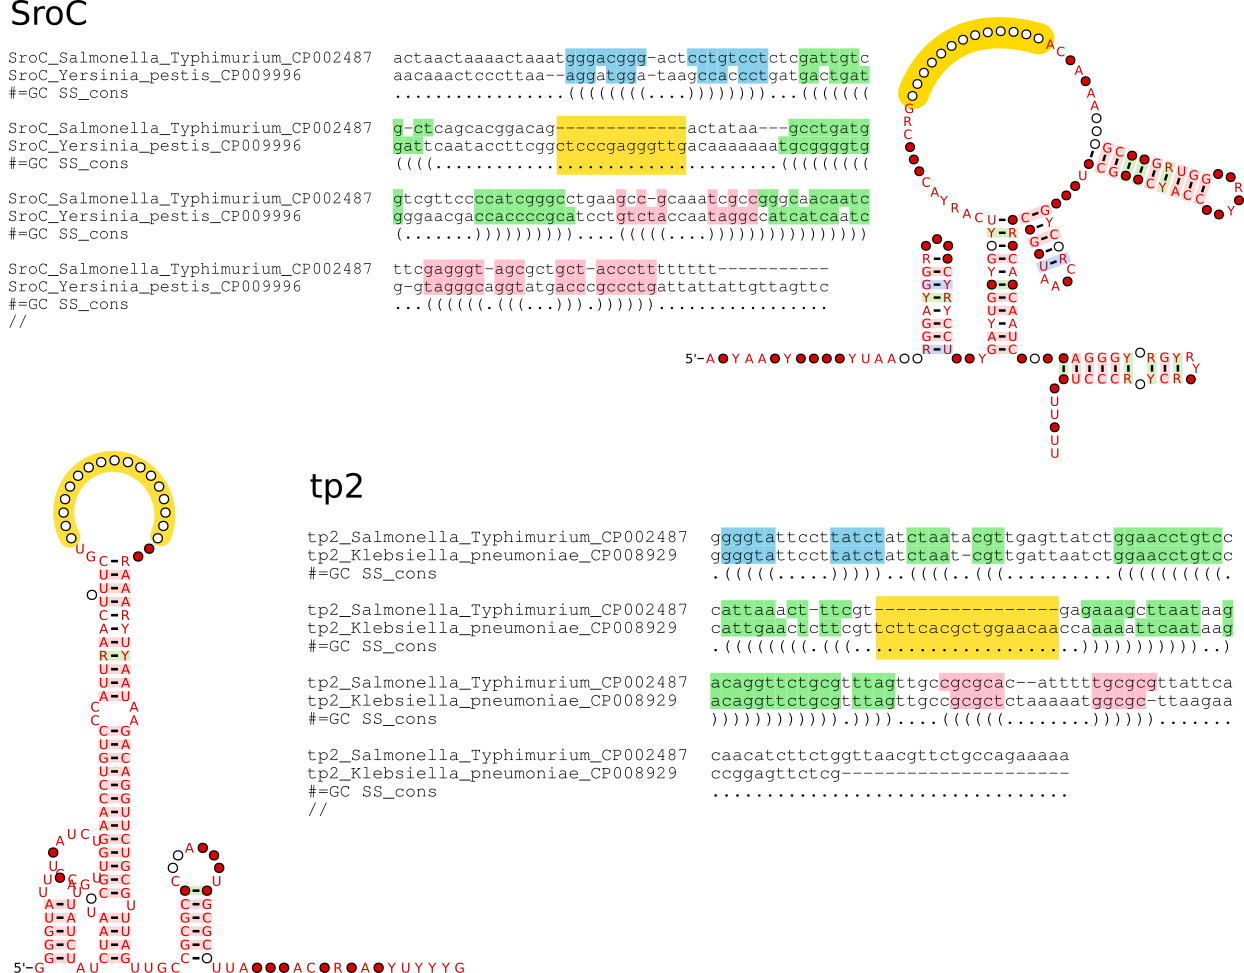
\includegraphics[scale=1.48]{sal/sroc_and_tp2.png}
    \caption[Examples of difficult to annotate ncRNAs]{Examples of difficult to annotate ncRNAs. These sequences contain large indels which make sequence alignment challenging. "Missing" intergenic sequences, consisting of the sequence located between flanking region annotations, and sequences annotated by the homology search were aligned using \texttt{mafft-qinsi}, and consensus secondary structure predictions generated with \texttt{RNAalifold}. \textbf{Top:} Alignment of \textit{tp2} from \textit{Salmonella} Typhimurium and intergenic sequence from the same locus in \textit{Klebsiella pneumoniae}. \textit{Bottom:} Alignment of \textit{SroC} from \textit{S.} Typhimurium and intergenic sequence from same locus in \textit{Yersinia pestis}. Bases are coloured by consensus structure using \texttt{RALEE} \citep{Griffiths2005-jojo}.}
     \label{fig:tp2_sroc_alignment}
\end{figure}

\subsection{Poorly conserved sRNAs are associated with horizontal gene transfer within \textit{Salmonella}}

Homology search results show that a large proportion of \textit{S.} Typhimurium ST4/74 sRNAs are \textit{Salmonella}-specific. Sixty sRNAs were found only in \textit{Salmonella}, 39 of which were annotated and highly conserved across all \textit{Salmonella} genomes. Twenty-one sRNAs were limited to \textit{S. enterica} subsp. \textit{enterica}, with \textit{STnc3800} being the only sRNA that was specific to \textit{S.} Typhimurium. 

Eighteen sRNAs were present only in \textit{S. enterica} subsp. \textit{enterica} within \textit{Salmonella}, but were also annotated in other genera. Annotations of surrounding proteins and genome comparisons found these sRNAs are associated with horizontal gene transfer events into \textit{Salmonella}, or are homologous to mobile genetic elements (Figures \ref{fig:inheritance_boxplot} and \ref{fig:hgt_detection} ). These include sRNAs found in large horizontally-acquired regions, such as prophages and pathogenicity islands, and sRNAs associated with transposons, insertion elements, and cryptic phages.

\begin{figure}[H]
    \centering
    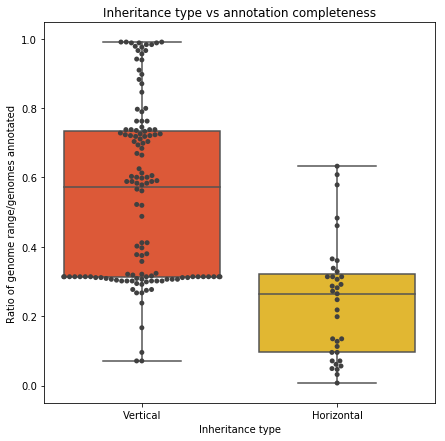
\includegraphics[scale=0.69]{sal/conservation_vs_inheritance_2.png}
    \caption[Conservation of sRNA sequences for different inheritance types]{Box-plot showing annotation density for sRNAs for horizontally-acquired and vertically inherited sRNAs. The y axis shows a ratio of annotated vs non-annotated genomes for an sRNA (all genomes for the genera containing at least one sRNA annotation). This shows that the proportion of genomes annotated is lower for horizontally-acquired sRNAs, as the mobile genetic elements are not consistently present in any lineage.}
    \label{fig:inheritance_boxplot}
\end{figure}

Many \textit{Salmonella} pathogenicity islands are horizontally transferred between strains or closely related species within \textit{Salmonella}. These islands are thought to be unique to the \textit{Salmonella} lineage, acquired after the \textit{Salmonella/E. coli} split several million years ago \citep{Baumler1997-xe}. Many pathogenicity islands appear to have a bacteriophage origin, and may have formed from phage sequence, or sequence laterally transferred by phage machinery \citep{Schmidt2004-js}. Several sRNAs located in pathogenicity islands appear to also have a phage origin, as they had homologous sequences in annotated prophages across the Enterobacteriaceae. 

Other \textit{Salmonella}-specific sRNAs did not have high sequence identity to MGE ncRNAs in other genera, but context such as surrounding protein-coding genes and analogous secondary structure \citep{Hershko-Shalev2016-kv} are indicative of a MGE origin. Many horizontally-acquired sRNAs were located within intact and cryptic transposons, such as  \textit{isrF}, which is located next to a frame-shifted transposase in \textit{S.} Typhimurium. The \textit{isrN} gene is located in between putative transposases; BLAST and Pfam annotations of the region encompassing \textit{isrN} and both flanking ORFs indicate that this is a frame-shifted IS3 transposase. The \textit{STnc490} sRNA (renamed \textit{tnpA}, previously \textit{art200}), which is located in the 5$\textprime$ UTR of IS200 transposons, has recently been identified as an important regulator of of pathogenicity in \textit{Salmonella} \citep{Ellis2018-zu,Ellis2017-uvv}. Transposon-derived sRNAs have also been introduced by \textit{Tn10/IS10} and \textit{Tn5/IS50} in \textit{E. coli} \citep{Ross2013-ee,Ross2014-ux,Ellis2015-we} suggesting that transposons may be a frequent source of ncRNA genes in these genera.

\subsection{Expression of conserved and horizontally-acquired sRNAs}

%https://www.ncbi.nlm.nih.gov/pmc/articles/PMC3677282/
%https://www.ncbi.nlm.nih.gov/pmc/articles/PMC4265352/
%https://www.ncbi.nlm.nih.gov/pmc/articles/PMC5006887/

Highly conserved sRNAs were also both highly and constitutively expressed across multiple growth conditions in experiments by \cite{Kroger2012-cr} and \cite{Kroger2013-pg}. Almost all of these sRNAs have verified interactions with the RNA-binding chaperones Hfq and ProQ \citep{Smirnov2016-yt,Holmqvist2016-hj} (shown in Figures \ref{fig:sal_heatmap}D and \ref{fig:sal_heatmap2}D), and are known to participate in complex regulons which influence essential stress responses and metabolic processes \citep{Updegrove2015-vu}.

The less well conserved vertically inherited \textit{Salmonella}-specific sRNAs were often poorly expressed, and often expressed in specific conditions. Few of these sRNAs have been experimentally verified or functionally characterised, however those exhibiting condition-specific expression presumably participate in or are linked to specific responses to the environment. 

Horizontally-acquired \textit{Salmonella}-specific sRNAs were generally highly and constitutively expressed, and few are predicted to bind to Hfq or ProQ. Non-coding RNAs contained within MGEs are often constitutively expressed. This may be to ensure dosage is sufficient when interacting with highly-expressed elements of the core genome, such as the Hfq-interacting sRNAs in \textit{E. coli} prophages \citep{Tree2014-xz}, and the \textit{Salmonella} SPI-1 sRNA InvR \citep{Pfeiffer2007-yb}. These sRNAs promote maintenance of the element by providing a beneficial phenotype to the host, which is best achieved by targeting genes which are themselves highly or constitutively expressed, allowing them to integrate into or form regulons essential for growth and survival \citep{Frohlich2016-pr,Pfeiffer2007-yb}. More well-known examples of MGE-encoded bacterial sRNAs are ncRNA repressors, which are highly expressed to suppress toxic effects of MGE genes, such as the phage-encoded IsrK \citep{Hershko-Shalev2016-kv}, or to act as antitoxins in addiction modules \citep{Lobato-Marquez2015-ah}. 

Genomic island sRNAs are generally expressed in specific growth conditions. While these sRNAs appear to have an MGE-origin, their relatively ancient association with \textit{Salmonella} may have allowed them to integrate with regulatory circuitry and take on more specific functions \citep{Frohlich2016-pr}.

\subsection{Vertically-inherited sRNAs are associated with integration}

The adjacent proteins for many highly conserved sRNAs (\textit{micA}, \textit{micC}, \textit{omrA}, \textit{omrB}, \textit{rybA}, \textit{rydC}, \textit{ryeC}, \textit{fnrS}) were sometimes annotated as MGE-like (i.e a transposase or integrase), which was infrequent and typically lineage-specific. The frequency of these annotations made it difficult to confidently assign inheritance type from functional annotations of nearby proteins alone (Figures \ref{fig:function_vs_inheritance} and \ref{fig:hgt_detection}).

Several vertically-inherited sRNAs were highly enriched for MGE insertion. The \textit{sdsR} gene has been identified as a phage insertion hot-spot in \textit{Salmonella} and \textit{E. coli} \citep{Balbontin2008-vv}, had 12.9\% of flanking protein annotations classified as MGE-like. MGE-like proteins were found near \textit{sdsR} in all enteric genera, indicating that \textit{sdsR} is also a preferred MGE insertion site outside of the \textit{Salmonella-Escherichia} lineage. Pathogenicity island sRNAs had varying proportions of nearby MGE-like protein annotations (\textit{STnc1710, STnc3870} in Figure \ref{fig:function_vs_inheritance}), due to the large size of these elements. 

The frequency and distribution of these annotations across the phylogeny suggest frequent insertion of transposable elements near sRNAs. An interesting example of a transposase insertion can be seen in \textit{spf}, which is located in a highly conserved ribosomal protein locus. In all \textit{Yersinia pestis} genomes in this study, \textit{spf} was next to an IS1541a transposase insertion. Some signals of past insertions can also be seen, for example the highly conserved iron-storage regulator \textit{fnrS} was located near a cryptic phage integrase in all \textit{Salmonella} and some \textit{E. coli} genomes in the data-set.


Some sRNAs are also located next to tRNAs, which are common insertion sites for phages and MGEs \citep{Reiter1989-nr,Williams2002-kj}. The \textit{glmZ} sRNA is located next to a tRNA locus, and is associated with integrases in strains from \textit{Salmonella}, \textit{Shigella} and \textit{Yersinia}. A recent example of this can be seen in \textit{S. enterica} sv. \textit{Montevideo}, where \textit{glmZ} appears to have been an insertion site for IS200. Poorly conserved sRNAs were also associated with insertions: the \textit{Salmonella}-specific \textit{isrO} sRNA, which is located next to a tRNA gene, is next to integrase annotations in \textit{Salmonella} Typhi, which is a recently diverged strain (\textasciitilde50,000 years old) \citep{Kidgell2002-hs}. 

\begin{figure}[H]
    \centering
        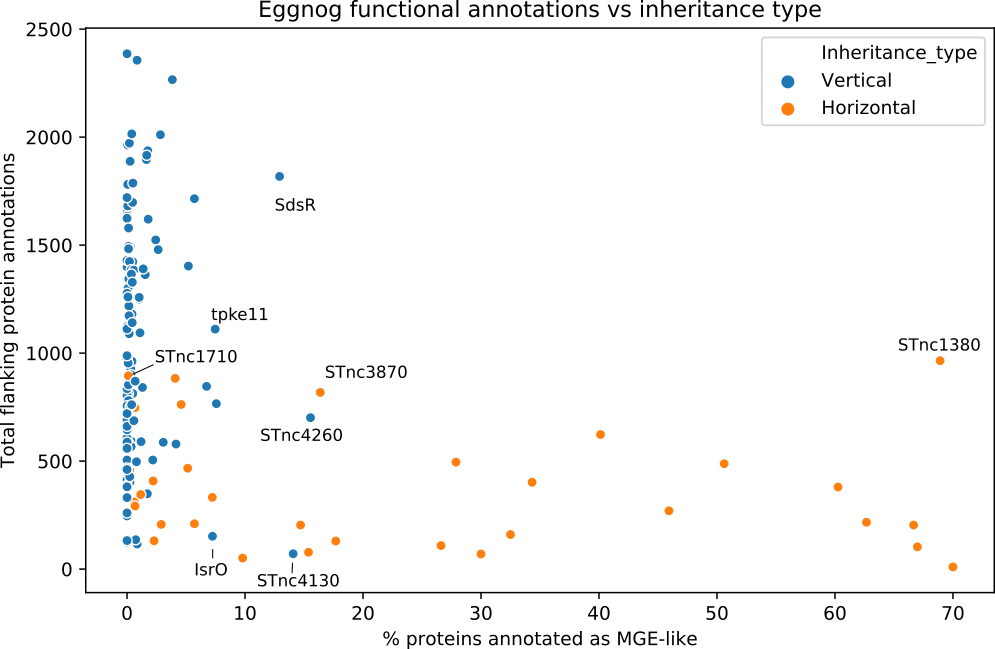
\includegraphics{sal/function_vs_inheritance_2.png}
    \caption[Association between flanking protein function and conservation]{Plot showing the association between sRNA flanking protein function and number of total number of annotations. Total annotations are for 6 proteins (+/-3 either side of the sRNA) per genome. Points for each gene are coloured by inheritance type. Most vertically inherited sRNAs have less than 0-5\% of flanking proteins annotated as MGE-like, and no vertically-inherited sRNAs have more than 20\% MGE-like flanking proteins. Horizontally-acquired sRNAs range from 0\% of proteins annotated as MGE-like, for sRNAs that are part of larger MGEs such as pathogenicity islands, to 70\% for sRNAs within transposition machinery. Several outliers from each inheritance type are highlighted, and are discussed in the text.}
    \label{fig:function_vs_inheritance}
\end{figure}
%L - Could be worth a figure showing the different contexts of some of these sRNAs, maybe as a companion panel to 1.11?
%CLIP-seq data set for ProQ published, this might be cleaner than the ProQ RIP in Smirnov et al. The paper’s here: https://www.sciencedirect.com/science/article/pii/S1097276518303137 let me know if you have any issues accessing the data. Some kind of enrichment or association testing on figs 1.7 and 1.8 might make the the association between conservation and expression / protein binding a bit more convincing


Many mobile genetic elements recognise specific sequence motifs as insertion sites, such as inverted repeats or tRNAs, which share similarities with structural components of sRNAs \citep{Darmon2014-dxjx, Siguier2014-jm,Williams2002-kj}. This has been proposed as the reason for phage insertion hotspots near \textit{cyaR}, which is an insertion site for phage P2 in \textit{E. coli} \citep{De_Lay2009-ye}. The frequent association between sRNAs and mobile genetic elements makes it difficult to untangle if these sRNAs are exapted from sequence motifs that permit MGE insertion, or are formed from remnants of previous HGT events \citep{Jose2019-wi}, as inverted repeats are both common within transposable elements and can be deposited within genomes by transposition \citep{Delihas2011-ra,Vandecraen2017-dh,Siguier2014-jm}.  

\subsection{Exaptation of sRNAs from type I toxin-antitoxin systems}

Type I toxin-antitoxin (TA) systems utilise sRNAs as antitoxins, which bind to toxin mRNAs to suppress toxin translation \citep{Brantl2012-ad}. Many of these are chromosomally encoded, and do not show classic signatures of horizontal gene transfer \citep{Fozo2010-xl,Coray2017-sb}. Several \textit{Salmonella} sRNAs are derived from Type I TA antitoxins, such as the \textit{rygC} and \textit{rygD} sRNAs (now renamed \textit{sibA} and \textit{sibC}), which are known homologues of the Sib RNA from Ibs-Sib TA systems in \textit{E. coli} K12 \citep{Hebrard2012-iy,Han2010-hn}. Homology search results found that \textit{STnc1420} also shares sequence similarity with annotated Sib RNAs in \textit{E. coli}. 

While the primary function of these sRNAs is to protect the host from the toxin, these regulons may also provide a fitness advantage. The \textit{Salmonella} IstR sRNA \citep{Vogel2004-ke}, which inhibits translation of its cognate TisB toxin, but IstR expression decreases during stationary phase, slowing growth as the toxin accumulates, which is thought to assist DNA repair. Recently, the SraC (aka RyeA) and SdsR sRNAs, which are transcribed from overlapping genes located on opposite strands, have been found to act as a novel type of entirely sRNA-based TA system in \textit{E. coli}, in which SdsR acts as a toxin by suppressing the translation of an inner membrane protein essential for growth \citep{Choi2018-sl}. Interestingly, this role does not appear to be conserved, as SdsR has different target ranges in \textit{E. coli} and \textit{Salmonella} \citep{Frohlich2016-pr}, and is also more highly conserved than its purported antitoxin SraC \citep{Frohlich2012-bf}.

The \textit{Salmonella} pathogenicity island sRNA \textit{isrA} was also found to share sequence similarity with the \textit{symE}-\textit{symR} TA system found in \textit{E. coli}. A previous BLAST-based study of sRNA turnover \citep{Skippington2012-iv} predicted \textit{isrA} homologues in \textit{E. coli} genomes, however \textit{isrA} was not found outside \textit{Salmonella} in this study after filtering. Examination of unfiltered homology search results showed multiple lower-scoring \textit{isrA} annotations in \textit{S. bongori} and \textit{S. arizonae} genomes.

Of the 6 candidate \textit{isrA} annotations in \textit{S. bongori} (NCBI accession CP006693), the majority were located opposite small hypothetical proteins in a Type VI secretion system. A BLAST search for these proteins returned results with \textasciitilde85\% sequence similarity to the \textit{E. coli} \textit{symE} toxin. A homology search of the \textit{S}. Typhimurium ST4/74 genome with HMMs of TA toxin proteins from \cite{Coray2017-sb} annotated the hypothetical proteins adjacent to \textit{isrA} as \textit{symE}, suggesting that \textit{isrA} may be derived from the sRNA antitoxin \textit{symR}. Previous annotation of TAs in \textit{Salmonella} Typhimurium \citep{Lobato-Marquez2015-ah} did not identify this \textit{symE} homologue with PSI-BLAST, however as with other sRNAs, the study and detection of Type I TA families is difficult due to the short and diverse RNA and protein-coding components \citep{Coray2017-sb}. 

\subsection{Conclusions and Future Directions}

We aimed to examine the rates of turnover of \textit{Salmonella} sRNAs using a sensitive iterative profile-HMM approach, which is effective at re-annotating known sRNAs from single starting sequences over large phylogenetic distances. These results confirm previous observations that sRNAs are both rapidly acquired and exhibit rapid sequence turnover. The incorporation of synteny anchors in this pipeline allowed us to resolve annotation conflicts, and predict that the limited phylogenetic distribution of many sRNAs is primarily due to gene gain and loss rather than sequence divergence. 

Many sRNAs contain secondary structure motifs in common with each other \citep{Gardner2015-cxxo}, and with other structured RNAs. This highlighted an additional challenge for sRNA homology search: reducing specificity is required to detect more distant homologues, but this can generate high rates of false positives, requiring careful filtering. This is further compounded by the short length of many sequences, making it easy for individual structural elements to return highly scoring results during homology search. 

With any nucleotide-based sRNA homology search, consideration of structural similarities to existing ncRNAs and evolutionary context, such as the presence of paralogues, is essential for studying rapidly evolving genes. Signals other than nucleotide sequence can be incorporated into homology search, for example 2D and 3D structure motifs for sRNAs containing conserved secondary structure \citep{Gardner2015-cxxo,Barquist2016-qt}. Genomic or syntenic context, such as the presence of conserved promoters or nearby proteins, is also useful in identifying highly divergent homologous sequences, however methods to incorporate this information are likely to be bespoke and difficult to scale \citep{Menzel2009-nxxs}, particularly for heterogenous genes such as bacterial sRNAs.

This study indicates that a large proportion of \textit{Salmonella enterica}-specific sRNAs (19/51) have been acquired \textit{via} horizontal gene transfer. While the classification of sRNAs into horizontally and vertically inherited is limited by our ability to detect signals of horizontal gene transfer over large periods of evolutionary time, it appears to horizontal gene transfer is the main driver of sRNA acquisition in \textit{Salmonella}. As we discussed previously \citep{Jose2019-wi}, exaptation of sRNA sequences introduced by horizontal gene transfer provides an easy way to integrate host and foreign DNA into regulons which benefit the host. Many sRNAs acquired by horizontal gene transfer interact with the core genome, as well as sRNAs which act to regulate HGT-acquired/derived elements \citep{Frohlich2016-mj} where sRNA regulation `tames' HGT-acquired genes \citep{Papenfort2010-cj}. 

The prevalence of `new' sRNAs that derive from toxin-antitoxin systems indicate another interesting route for acquiring new sRNAs through exaptation. It is thought that chromosomal Type I TA families spread by duplication; having multiple redundant TA systems may free an sRNA from strictly performing an antitoxin role, allowing it to be easily exapted \citep{Jose2019-wi}. The maintenance of orphan antitoxins sequences in the absence of its toxin counterpart may also be a useful defence against further TA integration, or provide redundancy for existing TAs.

We have also previously considered the likelihood of \textit{de novo} sRNA formation \citep{Jose2019-wi}. This study highlights many \textit{Salmonella} and some \textit{S.} Typhimurium-specific sRNAs that are vertically inherited, raising the question as to how these genes arose. Exploring the function and expression of these genes across \textit{Salmonella} sp. may clarify if these transcripts are conserved \textit{de novo} genes, or transcriptional noise in intergenic regions. 

Recent developments in methods for discovery and characterisation of bacterial sRNAs outside of the \textit{Escherichia-Salmonella} clade are rapidly increasing the number of sequences available for comparison. Experiments to identify and functionally characterise sRNAs in Yersinia sp. \citep{Yan2013-ga,Martinez-Chavarria2015-bh,Han2019-bg}, and more recently in \textit{Erwinia} \citep{Schachterle2019-rccq} and \textit{Edwardsiella} \citep{Gao2019-gh} are providing insight into sRNA sequence and functional conservation across phylogenetic distances that are poorly served by ncRNA homology search. Fine-grained studies of sRNA evolution remain lacking in other families, however recent efforts to characterise sRNAs in \textit{Pseudomonas} \citep{Pita2018-bxxi,Gomez-Lozano2012-xe,Gomez-Lozano2015-yx,Filiatrault2010-jmc} are likely to make between-family comparisons of sRNA turnover and evolution feasible in the near future. 

%\citep{Madera2008-gz} - profile comparer
%https://www.ncbi.nlm.nih.gov/pmc/articles/PMC3472101/
\bibliographystyle{otago}
\bibliography{sal_sRNA}